\subsection{Scene Navigation}

\TODO{RELATE THESE TO PROJECT IN DISCUSSION}


% SCENE NATIGATION

Following is a list o scene navigation solutions.
Each one can contribute to a more powerful and easy interface.


\subsubsection{Smart and Physically Based Camera, 2006}
\label{SMARTCAM-LABEL}

In order to ensure users not ``getting lost'' in the virtual space,
Buchholz, Bohnet and D�llner \cite{SMARTCAM} propose a smart and physically based camera.
Smart in the sense that it is aware of confusing and disorienting viewing situations,
providing means to circumvent them.
Physically based because it is supported by a physics model of 3D motion
to ensure steady, continuous user movements.

Experience shows that people frequently lose track of their location when moving on a 3 dimensional
world.
To solve this problem, the camera must identify situations when to intervene.
For that reason a metric, called orientation value, was created.
Each view is classified by counting its pixels, granting different values:
landmarks get the highest values; terrain gets mid-range values and the sky gets lower values (see Fig. \ref{FIG-SMARTCAM1}, right).
A threshold can then be established and views below the threshold are classified ``disoriented''.
When such an event takes place, smart navigation techniques restrict camera control.
The constraints posed to user control must be as comprehensible as possible.
Camera movement should also be time-coherent and physically sound.

The maintenance strategy solves critical situations such as (see Fig.\ref{FIG-SMARTCAM1}, left):

\begin{enumerate}[a)]
	\item The user rotates the flight direction and causes the camera to look too far beyond the terrain border.
		The rotation is accepted but outweighed by a slight rear movement away from the border.
	\item The user is flying forward beyond the terrain border.
		The maintenance strategy temporarily tilts down the view direction until a maximum angle is reached.
	\item If no more tilting is possible, the strategy rotates the flight direction parallel to the terrain
		to fly along the terrain border.
\end{enumerate}

\begin{figure}[!ht]
	\centering
	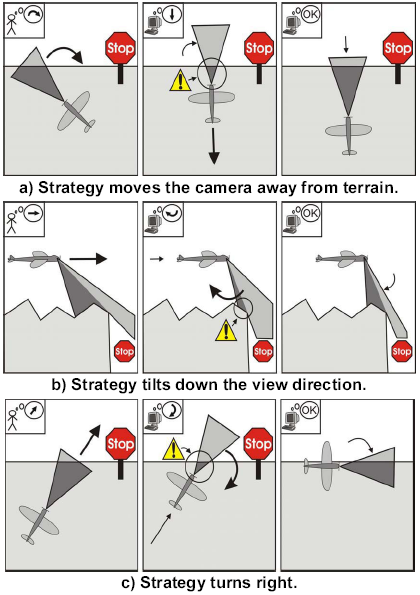
\includegraphics[height=7cm]{gfx/smartcam05-1.png}
	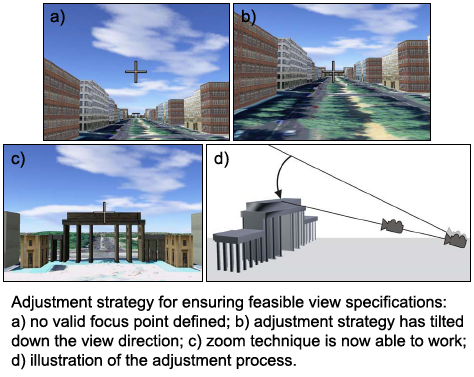
\includegraphics[height=5cm]{gfx/smartcam05-2.png}
	\caption{SPB Cam: Maintenance strategy for keeping high orientation values; Adjustment strategy for ensuring of feasible view specifications.}
	\label{FIG-SMARTCAM1}
\end{figure}

%\paragraph{Discussion}

A camera system such as this can be useful aiding non-experienced users such as clients in navigation tasks
since it maximizes the presence of landmarks in the user's view.
The physically-based engine would grant additional realism to the navigation experience, providing collision
detection, inertia and a spring behavior that would soften camera trajectories.

%\TODOL{RELATE TO PROJECT}


\subsubsection{Speed-dependent Automatic Zooming, 2000}
\label{SPEEDZOOM-LABEL}

Igarashi and Hinckley \cite{SPEEDZOOM} propose a simple idea for scrolling through large areas of information.
The speed at which the scrolling occurs changes the zooming of the seen area.
This makes sense since the faster the area is scrolling, the longer ahead the user needs to see.

%\paragraph{Discussion}

This could be easily applied to bird's-eye-view maps of large areas.
The scrolling of the map would trigger different zooming factors depending on
the scrolling speed, improving the navigation and exploration of the map.

%\TODOL{CAN THIS BE APPLIED?}


\subsubsection{Path Drawing for 3D Walkthrough, 1998}
\label{PATH3D-LABEL}

Igarashi et al. \cite{PATH3D} start by identifying the two main types of walkthrough techniques:
\emph{driving}, where the user continuously changes camera position with move and rotation buttons and
\emph{flying}, where the user picks the desired destination with a pointing device and a trajectory is calculated
and animated from the starting position to the picked one.
Each has it disadvantages:
driving requires the user to control the trajectory at all times;
flying lacks expressive power since the user can't control the path neither the final orientation.

The proposed solution is an extension of the flying technique:
the user draws the desired path he wants to take on the screen.
It gets projected onto the walking surfaces and the generated path is animated.
During the animation the user faces the tangential direction related to the path.
This brings the additional advantage of the user being able to define
where he will be facing at the end of the animation.
This technique can be used is two different ways.
The user can draw a long stroke specifying the path at once
or he can draw successions of small strokes (see Fig.\ref{FIG-PATH3D}).

As limitations the authors state the path expressiveness
being limited to the walking surface planes
and the need for the user's avatar to be present on the view
if one wants to draw the path from the user's feet.
 

\begin{figure}[!ht]
	\centering
	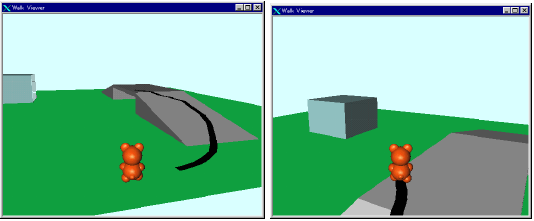
\includegraphics[width=12cm]{gfx/path3d.png}
	\caption{One long path and one short one}
	\label{FIG-PATH3D}
\end{figure}

%\paragraph{Discussion}

This navigation mode could be handy in the review scenario.
Even so this might be hard to apply to the project due to LSD interface limitations.